\documentclass[Thesis.tex]{subfiles}
\begin{document}

\chapter{The {\sc Jtem} libraries {\sc HalfEdge} and {\sc HalfEdgeTools}}

This chapter describes the {\sc Java} implementation of a half-edge data structure and a set of tools
combined in the package {\sc HalfEdgeTools}. Both packages are part of the {\sc Jtem} project
\cite{JtemWebsite}. This is joint work with Boris~Springborn ({\sc HalfEdge}), Thilo~R{\"o}rig, 
Felix~Kn{\"o}ppel, and Kristoffer Josefsson ({\sc HalfEdgeTools}), and
other contributers to the {\sc Jtem} project.

This particular implementation of a half-edge data structure was inspired by an implementation 
contained in the {\sc Cgal} library \cite{Kettner2000}.
This specific implementation is however different from existing libraries as is uses the generic
programming concept of {\sc Java} to achive compatibility and flexibility.

The code presented in this section is compatible with {\sc Java} version 1.7 or later.

\label{sec:halfedge_halfedgetools}
\section{The {\sc HalfEdge} data structure}

Half-edge data structures are used primarily to represent cell decompositions of oriented surfaces.
We say "primarily" because half-edge data structures can be used to represent somewhat more general
combinatorial structures, such as, for example, a checker board surface with white squares removed.

Here, surface means two-dimensional manifold, possibly with boundary; and a cell decomposition 
of a surface is a graph embedded in the surface such that the complement of the graph is 
(topologically) a disjoint union of open disks. The term map on a surface means the same. 
Thus, a cell decomposition decomposes a surface into vertices, edges, and faces.

{\bf Regular and strongly regular}

A cell decomposition of a surface is called regular, if it has no loops (edges with the same vertex 
on both ends), and if the boundary of a face contains an edge or vertex at most once. It is called 
strongly regular if two edges have at most one vertex in common, and if two faces have at most 
one edge or one vertex in common. A strongly regular cell decomposition is usually called a mesh.

{\bf This half-edge data structure implementation}

This half-edge data structure implementation consists of different types of objects representing 
vertices, half-edges, and faces. The term half-edge can and should be thought of as synonymous
with oriented edge or directed edge.

Every half-edge object holds references to:

\begin{itemize}
\item its oppositely oriented companion edge
\item the next edge in the boundary of the face on its left hand side
\item the previous edge in the boundary of the face on its left hand side
\item the face on its left hand side
\item the vertex it points to.
\end{itemize}

The face and vertex objects hold back references to a half-edge referencing them. Finally, there 
is the class {\tt de.jtem.halfedge.HalfEdgeDataStructure} representing a whole half-edge data 
structure. It acts as a container for (and sort of factory of) its vertices, half-edges, and faces.

{\bf Use of Generics}

Typically, one wants to equip vertices, edges, and faces with additional properties or functionality. 
For example, vertices may have coordinates associated with them, edges may have weights, and 
faces may have colors.

Our half-edge data structure facilitates this by using generic classes as abstract base classes for 
vertex, edge, and face types: The classes {\tt de.jtem.halfedge.Vertex}, {\tt de.jtem.halfedge.Edge}, 
{\tt de.jtem.halfedge.Face} are all parameterized with the associated vertex, edge, and face types.

{\bf Example}

To create a half-edge data structure with vertices that have 2D coordinates, proceed as follows.

\begin{itemize}
\item{Step 1.} 
Define appropriate subclasses of {\tt de.jtem.half\-edge.Vertex}, {\tt de.jtem.half\-edge.Edge}, and 
{\tt de.jtem.halfedge.Face}, for example:

\begin{lstlisting}[numbers=none]
public class MyVertex extends Vertex<MyVertex, MyEdge, MyFace> {
	public Point2D p;
}
public class MyEdge extends Edge<MyVertex, MyEdge, MyFace> { }
public class MyFace extends Face<MyVertex, MyEdge, MyFace> { }
\end{lstlisting}

Of course you might make the property {\tt p} of {\tt MyEdge} private and provide getter and setter 
methods, etc. Note that you always have to subclass {\tt de.jtem.half\-edge.Vertex}, 
{\tt de.jtem.half\-edge.Edge}, and {\tt de.jtem.half\-edge.Face}, even if you do not define any 
additional functionality or properties.

\item{Step 2.} 
Instantiate a {\tt de.jtem.halfedge.HalfEdgeDataStructure}:

\begin{lstlisting}[numbers=none]
HalfEdgeDataStructure<MyVertex, MyEdge, MyFace> heds = new HalfEdgeDataStructure<>(MyVertex.class, MyEdge.class, MyFace.class);
\end{lstlisting}

The parameters of the constructor serve as run time type tokens. Alternatively you can create a subclass
of {\tt de.jtem.halfedge.HalfEdgeDataStructure} and create an instance of this:

\begin{lstlisting}[numbers=none]
public class MyHDS extends HalfEdgeDataStructure<MyVertex, MyEdge, MyFace> {
	public MyHDS() {
		super(MyVertex.class, MyEdge.class, MyFace.class);
	}
}
...
MyHDS mds = new MyHDS();
\end{lstlisting}

\item{Step 3.} 
Instantiate vertices, edges, and faces using the {\tt addNewVertex}, {\tt addNewEdge}, and 
{\tt addNewFace} methods, like this:

\begin{lstlisting}[numbers=none]
MyVertex v = heds.addNewVertex();
MyEdge e = heds.addNewEdge();
MyFace f = heds.addNewFace();
\end{lstlisting}

\end{itemize}

{\bf Linkage and incidence.}

Node classes provide methods to create a valid data structure. Most of the methods are bidirectional linkage methods that affect the target and the caller. The corresponding methods are:
\begin{itemize}
\item {\tt E.linkNextEdge} sets the {\tt nextEdge} property of this edge as well as the 
{\tt previousEdge} property of the given edge.
\item {\tt E.linkOppositeEdge} sets the {\tt oppositeEdge} property of this edge and of the given edge accordingly.
\item {\tt E.linkPreviousEdge} sets {\tt previousEdge} and {\tt nextEdge} properties of this and the given edge.
\item {\tt E.setLeftFace} sets the {\tt leftFace} property of this edge and the {\tt boundaryEdge} property of the given face.
\item {\tt E.setTargetVertex} sets the {\tt targetVertex} property of this edge and the 
{\tt incommingEdge} property of the given vertex.
\end{itemize}

{\bf Node indices.}

During algorithm development it is often necessary to access consistent indices on vertices,
half-edges, or faces. We support this operation by the {\tt index} field of nodes accessible via
the {\tt getIndex()} method of all node types. Nodes are required to have indices $0,\ldots,\#V$,
$0,\ldots,\#E$, and $0,\ldots,\#F$ respectively. Note that $\#E$ is the number of half-edges
in the data structure. The running time of a {\tt getIndex} operation is $\mathcal{O}(1)$ if
no {\tt remove} operation has invalidated the indices. Otherwise it is $\mathcal{O}(n)$ where
$n$ is the numer of nodes in the data structure, e.g., $n=\#V$.

{\bf Iterating and directly accessing nodes.}

Nodes can be directly accessed via the corresponding {\tt get} method. It takes the node index
and returns the node with the given index. It is guaranteed that for a given $i\in \{0,\ldots,\#N\}$
it is {\tt getNode($i$).getIndex()$ = i$}.
Nodes in the data structure can be interated over using one of the methods {\tt getVertices}, 
{\tt getEdges}, or {\tt getFaces}. These return unmodifyable instances of {\tt java.util.List} containing the respective node instances.

{\bf Undirected edges}

A half-edge has the {\tt positive} property. In a pair of opposite edges it is required that the boolean
value of this property is different, i.e., \url{e.isPositive()} $!=$ \url{e.getOppositeEdge().isPositive()}.
Using this property it is possible to iterate over undirected edges, i.e., the positive or the negative
haf-edges. The methods {\tt getPositiveEdges} and {\tt getNegativeEdge} of the data structure 
implement this.

{\bf Removing nodes from a data structure.}

A node can be deleted from the data structure using the {\tt removeVertex/Edge/Face} methods.
The running time of a remove operation is always $\mathcal{O}(1)$. Node indices however will
get invalidated and reindexed on the next access of any index related operation that in turn will
then have running time $\mathcal{O}(n)$.

{\bf Half-Edge utilities.}

To work efficiently with half-edge data a set of algorithms is implemented as static ulitity methods
in the class {\tt de.jtem.half\-edge.util.Half\-Edge\-Utils}. It contains methods that help iterating 
over incoming edges at a vertex, or iterating over the boundary edges of a surface or a face, and many more.


\section{Data, Algorithms and Tools}

A set of algorithms and tools is implemented in the {\sc Jtem} project {\sc HalfEdgeTools}
\cite{JtemWebsite}. 

Many algorithms in the library are purely combinatorial. This means there is no extra data 
involved during algorithm execution. Thus such an algorithm is generic by definition. The
method signature could look like this:

\begin{lstlisting}
public static <
	V extends Vertex<V, E, F>,
	E extends Edge<V, E, F>,
	F extends Face<V, E, F>,
	HDS extends HalfEdgeDataStructure<V, E, F>
> void triangulate(HDS hds){
	...
}
\end{lstlisting}

This method works on any half-edge data structure that is either an instance of {\tt
de.jtem.half\-edge.HalfEdgeDataStructure} or an instance of a sub-class. This method
signature makes the algorithm code itself look very clean. For instance iterating over
all vertices amounts to:

\begin{lstlisting}
for (V v : hds.getVertices()) {
	E e = v.getIncomingEdge();
	...
}
\end{lstlisting}

On the other hand when designing a generic algorithm that needs certain data associated
with nodes we have basically two options. Option 1. requires the generic node classes to
implement the required interfaces:

\begin{lstlisting}
public static <
	V extends Vertex<V, E, F> & HasCoordinate3D,
	E extends Edge<V, E, F>,
	F extends Face<V, E, F>,
	HDS extends HalfEdgeDataStructure<V, E, F>
> void convexHull(HDS hds){
	...
	Coordinate3D x = v.getCoordinate3D();
}
\end{lstlisting}

This forces the Vertex implementations that use this algorithm to implement an interface
called {\tt HasCoordinate3D}. It leads to explicit and clean code of the algorithm. A drawback of this
is that an existing implementation that should use this algorithm has to be adapted to implement the 
possibly many interfaces required by the algorithm. 
This is not a feasable solution when is comes to a modular application where algorithms come as 
plug-ins without the chance to change the data structure.

{\bf AdapterSet and Adapters}

The second option uses the concept of adapters and is implemented in the package {\tt
de.jtem.\-halfedge\-tools.adapter}. An adapter defines a map from nodes to a data type supported 
by the adapter. We first show how this concept works when designing algorithms and then
describe the implementation of the required adapters. 

In this next example we calculate the discrete Dirichlet energy of a double valued function with 
double valued weights on edges. 

\lstinputlisting[
	caption={Algorithm that uses data from the {\tt AdapterSet}. The {\tt get} method of the
		{\tt AdapterSet} takes the data class type to find a matching adapter (Line~12 and 13).
		The corresponding {\tt getDefault} method takes a default value that is returned if no
		matching adapter is found (Line~14). It uses {\tt @FunctionValue} and {\tt @Weight} annotated 
		adapters to aquire the data needed for calculation of the output value.
	},
	label=alg:dirichlet,
	captionpos=b,
	firstline=14,
	lastline=31
]{java/de/sechel/thesis/MyUtility.java}

This method requires the {\tt AdapterSet} to contain adapters that provide
{\tt @FunctionValue} data on vertices (Line~12 and 13) and {\tt @Weight} data on half-edges (Line 14). 

The classes {\tt FunctionValue} and {\tt Weight} are runtime annotation classes, e.g.,

\begin{lstlisting}
@Retention(RetentionPolicy.RUNTIME)
@Target(ElementType.TYPE)
public @interface FunctionValue {}
\end{lstlisting}

An adapter class annotated with this annotation serves as {\tt @FunctionaValue} data adapter when 
called for as in Line 11-13 of Listing~\ref{alg:dirichlet}. The meaning of adapter annotations is 
an agreement between the algorithm using it and the implementor of the adapter. It is subject
of a best-practice policy to implement the adapters such that they output data that fit its 
annotation names.

There are three basic classes that could serve as base class of an adapter. It is

\begin{itemize}
\item {\tt Adapter} - The abstract base class of all adapters. Should never be subclassed directly.
\item {\tt AbstractAdapter} - A adapter class that knows about the supported data type and implements
all getter and setter methods. Here only the needed methods can be overwritten. Node type checking
is done manually thus allows for the creation of generic adapters.
\item {\tt AbstractTypedAdpter} - If you know which half edge node classes the adpter is supposed to
work with this is the adapter base class you should use. Node type checking and casting is done in the
super class.
\end{itemize}

An adapter implementation using the {\tt AbstractAdapter} is for instance:

\lstinputlisting[
	caption={
		Adapter implementation using the {\tt AbstractAdapter} as base class and a 
		map as storage concept for double values on generic vertices. It is annotated 
		with a {\tt @FunctionValue} annotation to serve as
		provider for data in the {\tt AdapterSet} (Line 1). The super class {\tt
		AbstractAdapter} is parameterized with the data type of the implementation; In this
		case {\tt Double} (Line 2). 
		The super class constructor is invoked with the class object of this type and flags 
		that tell the adapter
		if get and/or set operations are permitted (Line 6). The method {\tt canAccept}
		decides whether the adapter can work with the given node class; In this case the 
		adapter can accept any {\tt Vertex} object (Line 12). 
		Vertex getter and setter methods are generic methods (Line 16 to 32). 
	},
	label=lst:adapter,
	captionpos=b,
	firstline=13,
	lastline=50
] {java/de/sechel/thesis/MyAbstractAdapter.java}

When writing the adapter for concrete node classes we have a more concise description:

\lstinputlisting[
	caption={
		An adapter using {\tt AbstractTypedAdpter} as base class. Also annotated with the {\tt
		@FunctionValue} annotation. This super class is parameterized
		with a set of node class implementations and the adapter data type. Here the super
		constructor takes the node class objects or {\tt null} if a node type is not supported, the
		data type class object, and the getter/setter flags. The vertex getter and setter methods 
		are not generic and the corresponding casting is done in the super class. Adapters working
		on edges or faces implement the corresponding {\tt get/setEdgeValue} or 
		{\tt get/setFaceValue} methods.
	},
	label=lst:adapter,
	captionpos=b,
	firstline=9,
	lastline=50
] {java/de/sechel/thesis/MyTypedAdapter.java}

Using this concept of typed adapters the usage of an algorithm amounts to the implementation of
required data adapters and the creation of a suitable {\tt AdapterSet}.

\lstinputlisting[
	caption={Usage example of the algorithm presented in Listing~\ref{alg:dirichlet}. In this example 
	an empty data structure is created, filled with a dodecahedron combinatorics, and then processed by the 	
	algorithm. The {\tt AdapterSet} contains the {\tt @FunctionValue} annotated adapter to provide 
	{\tt Double} values on vertices. In this example a {\tt @Weight} adapter in not needed since the 
	{\tt computeDirichlet} algorithm uses the {\tt getDefault} method to obtain weight data for edges.},
	label=alg:dirichlet,
	captionpos=b,
	firstline=33,
	lastline=40
]{java/de/sechel/thesis/MyUtility.java}

{\bf Generic Adapters}

There is a set of generic adapters implemented in the package 
{\tt de.jtem.half\-edge\-tools.adap\-ter.generic}. Here generic means that the adapter does not provide
the data itself. Instead it asks for other adapters to provide data and converts, merges, or recalculates its
output based on the data aquired from other adapter implementations.

The most important example of pre-defined generic adapters are position and texture position adapters.
These adapters come in three versions, e.g., {\tt @Position2D}, {\tt @Position3D}, and {\tt @Position4D}. The implementations, e.g, {\tt de.jtem.half\-edge\-tools.adapter.generic.Position\-3dAdapter} obtain position
data from the {\tt AdapterSet} using the adapter annotated with {\tt @Position} and convert if the lengths
of arrays is not equal to $3$.

An algorithm using generic adapters is free of data conversion code.


{\bf Error Handling}

If a data adapter that is used by an algorithm is not found, the {\tt AdapterSet} throws exceptions stating
the name of the required annotation and the node type that is expected. 

\begin{lstlisting}[
numbers=none, stringstyle=\ttfamily,keywordstyle=\ttfamily, numbersep=0pt,xleftmargin=20pt
]
Exception in thread "main" de.jtem.halfedgetools.adapter.AdapterException: Adapter "FunctionValue" for node VV not found
	at de.jtem.halfedgetools.adapter.AdapterSet.get(Unknown Source)
	at de.sechel.thesis.MyUtility.computeDirichlet(MyUtility.java:25)
	at de.sechel.thesis.MyUtility.calculate(MyUtility.java:39)
	at de.sechel.thesis.MyUtility.main(MyUtility.java:44)
\end{lstlisting}


\section{{\sc HalfEdgeTools} and {\sc Jreality}}

The {\sc HalfEdgeTools} package contains utility classes for the visualization of half-edge data with 
{\sc Jreality} \cite{JrealityWebsite}. It is part of the {\sc Jtem} project \cite{JtemWebsite}. 

{\bf Half-edge Interface}

A central role plays the plug-in {\tt de.jtem.halfedge\-tools.plugin.Halfedge\-Interface}. This plug-in works 
as a converter between half-edge data structure and {\tt IndexedFaceSet} data structure used internally 
by {\sc Jreality}. It creates a user interface that contains gui elements for layer management, import, export,
undo, redo, and more features, see Figure~\ref{fig:halfedge_interface}.

\begin{figure}
	\centering
	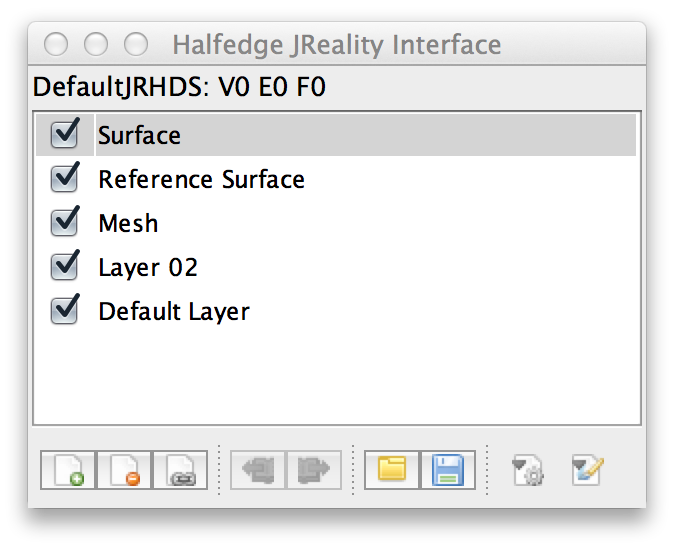
\includegraphics[width=5cm]{jrworkspace/halfedge_interface_hires.png}
	\caption{The user interface created by the {\tt HalfedgeInterface} plug-in. It manages layers that
		contain different instances of half-edge data structures and the corresponding visualizations.
		Layers can be merged, {\tt OBJ} files can be exported and imported and visualization
		options can be adjusted. 
	}
	\label{fig:halfedge_interface}
\end{figure}

The API of the {\tt HalfedgeInterface} supports {\tt set} and {\tt get} methods that convert to and from
{\sc Jreality}. During conversion data is read from an {\tt AdapterSet} that is managed by the half-edge
interface. The plug-in supports various data on node types. We give a list of annotation types and
their purposes. All conversion adapters work with {\tt double[]} or {\tt double} data types. All
supported annotation types are in the package {\tt de.jtem.halfedgetools.adapter.type}.

\begin{itemize}
\item {\tt\bf @Position} - Positions of vertices can have lengths 2, 3, or 4.
\item {\tt\bf @Color} - Colors either on vertices, edges, or faces.
\item {\tt\bf @Normal} - Normals usually for vertices or faces.
\item {\tt\bf @TexturePosition} - Texture coordinates of length 2, 3, or 4.
\item {\tt\bf @Label} - Text annotations that appear next to the node.
\item {\tt\bf @Radius} - Radii of vertex sphere representations or edge cylinders when rendered
as spheres or tubes.
\item {\tt\bf @Size} - Size in pixels of vertex points or edge lines when rendered as points or lines.
\end{itemize}

Internally the conversion is done using the classes from the package 
{\tt de.jtem.halfedge\-tools.jreality}. Conversion from and to a {\sc Jreality} {\tt IndexedFaceSet}
is implemented in {\tt ConverterHeds2JR} and {\tt ConverterJR2Heds}.

{\bf Visualization Interface}

A second important plug-in is the {\tt Visuali\-zation\-Inter\-face}. It defines
an plug-in API and various implementations for data visualization with the half-edge data structure. 


\begin{figure}
	\centering
	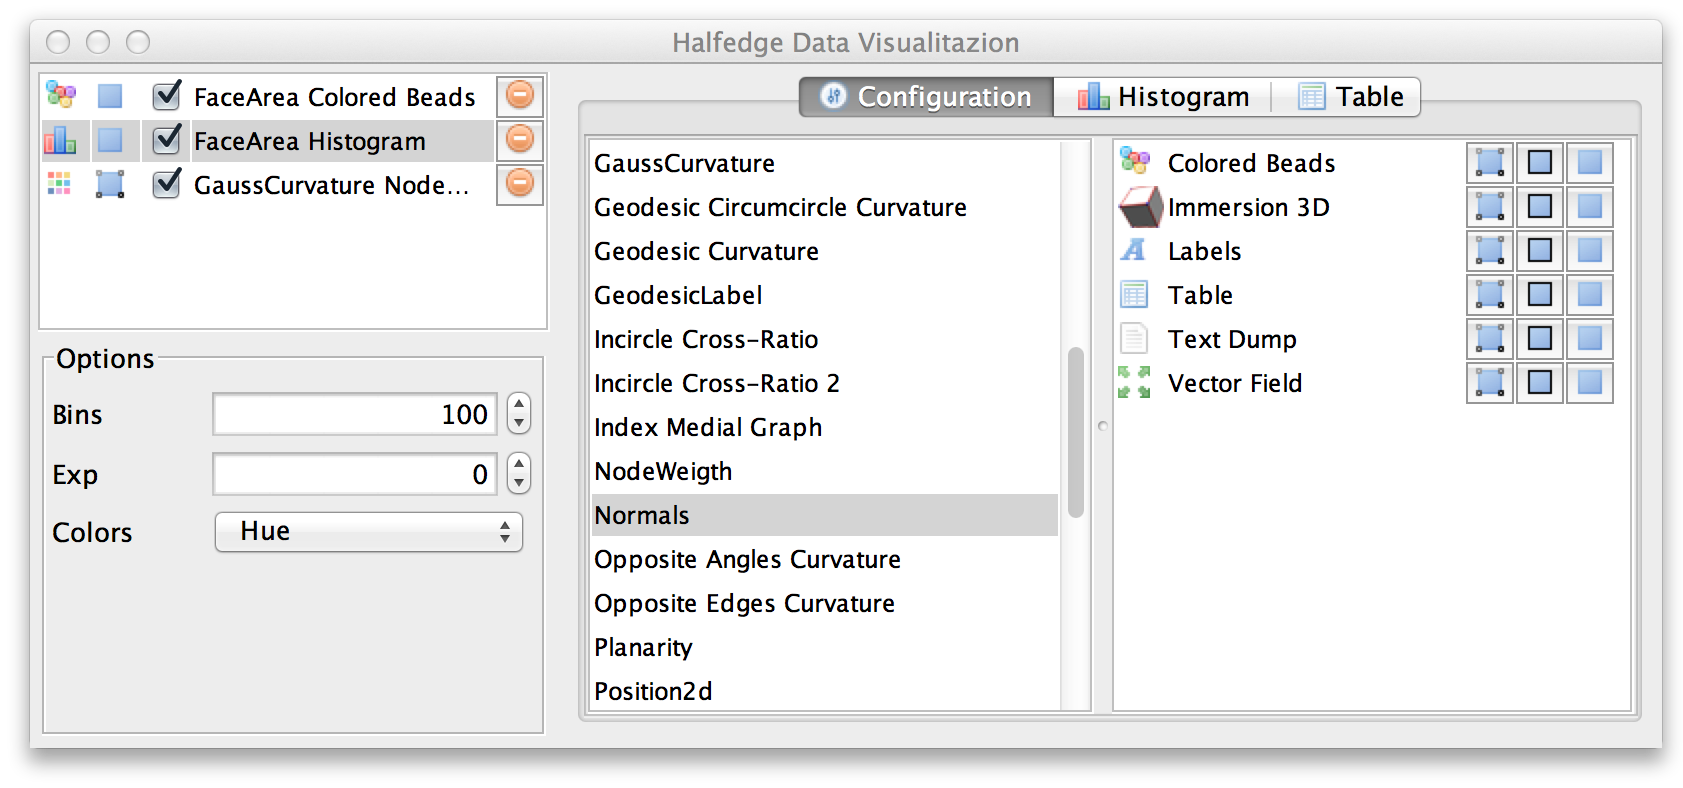
\includegraphics[width=11cm]{jrworkspace/visualization_interface_hires02.png}
	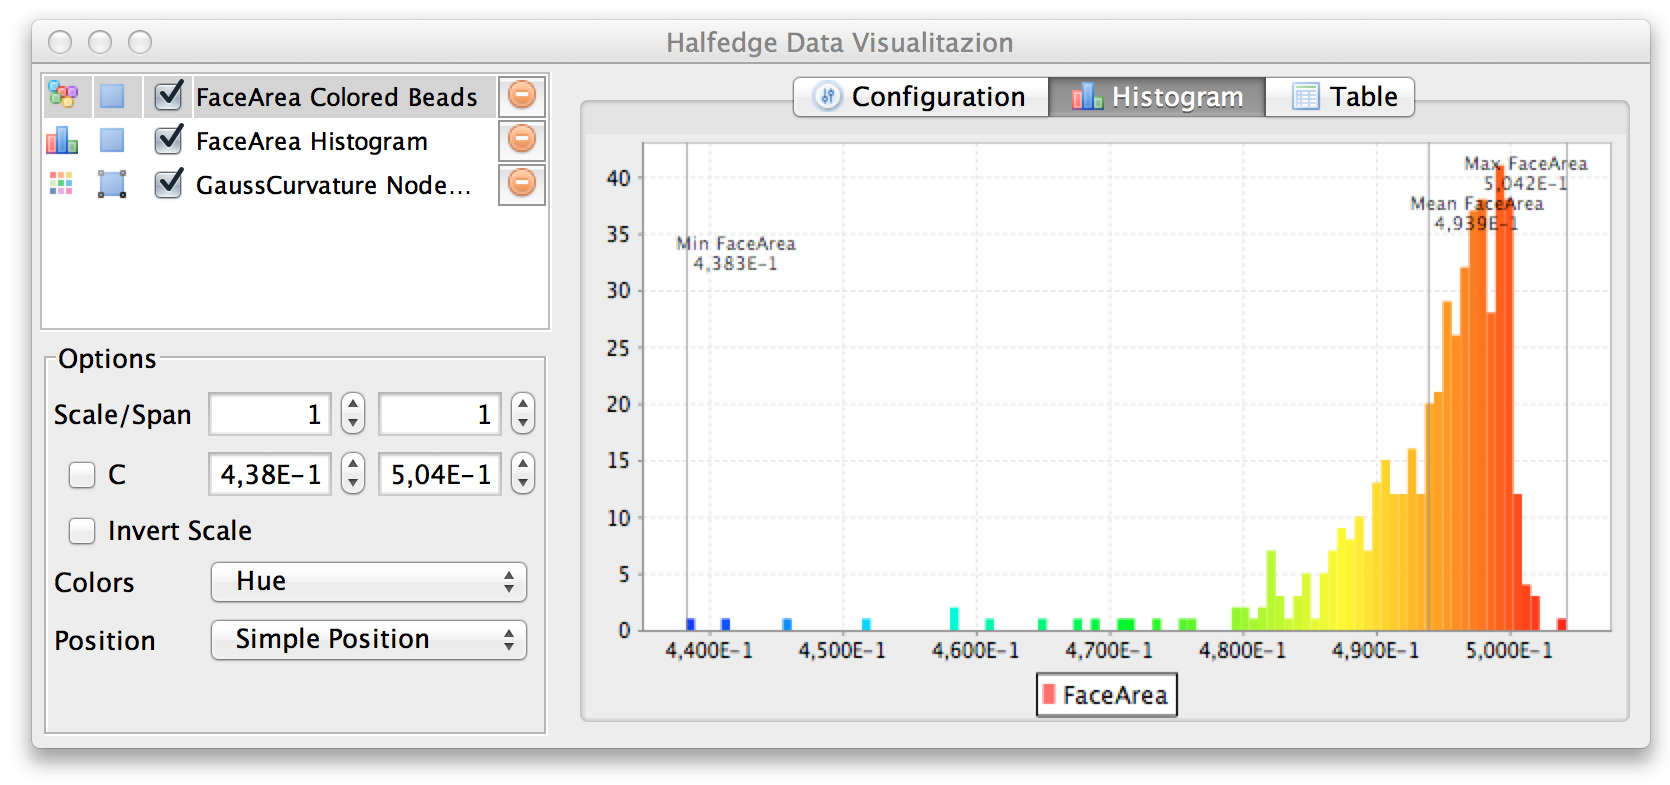
\includegraphics[width=11cm]{jrworkspace/visualization_interface_hires.png}
	\caption[Visualization Interface]{The half-edge visualization user interface. Selection of a visualization
		plug-in for a data adapter (top). A histogram view for scalar data on half-edge nodes (bottom).}
	\label{fig:visualization_interface}
\end{figure}

Every {\tt Adapter} that is managed by the {\tt HalfedgeInterface} is available as data source. In 
addition to this every plug-in extending {\tt de.jtem.half\-edgetools.plugin.data.Data\-Source\-Provider} 
is asked for data adapters. A list of these data sources is displayed in the user interface, see 
Figure~\ref{fig:visualization_interface} (top). A visualization of the selected data source is created by a
corresponding {\tt DataVisualizer} plug-in. For scalar data on vertices, edges, or faces we provide the 
colored beads visualizer or simply colored nodes, Figure~\ref{fig:visualizers}. There is a histogram that displays a density
plot for scalar data on nodes, Figure~\ref{fig:visualizers} (right) and Figure~\ref{fig:visualization_interface} (bottom). For vector valued data 
there is a visualizer that creates arrows starting at half-edge nodes.


\begin{figure}
	\centering
	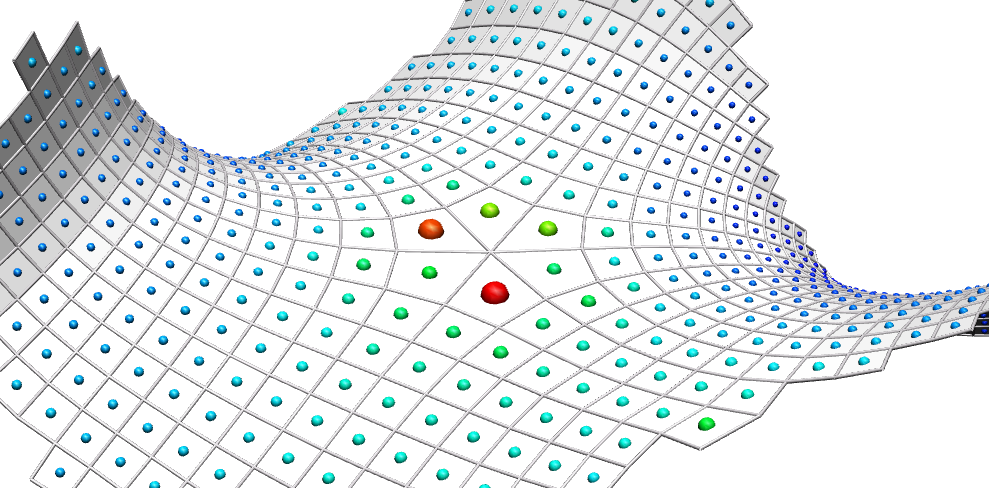
\includegraphics[width=4.5cm]{jrworkspace/colored_beads.png}
	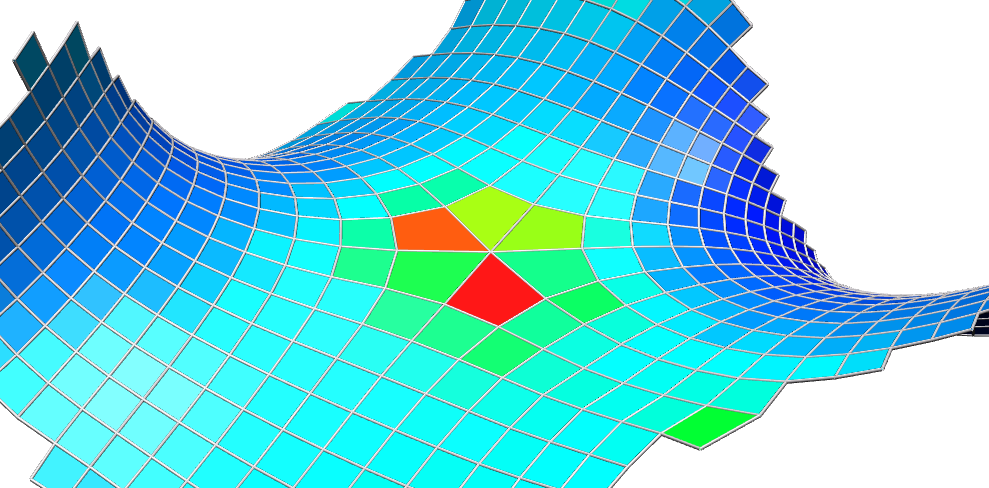
\includegraphics[width=4.5cm]{jrworkspace/node_colors.png}
	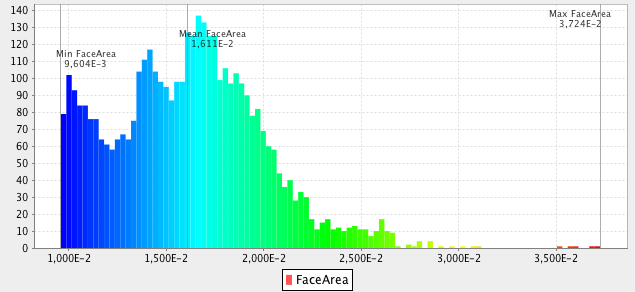
\includegraphics[width=5cm]{jrworkspace/histogram.png}
	\caption[Visualizers]{Different visualization plug-ins for scalar data on faces. Colored beads (left),
		node colors, and histogram view.}
	\label{fig:visualizers}
\end{figure}

\subfilebibliography
\end{document}

%%% Local Variables:
%%% TeX-master: "Thesis.tex"
%%% End: